% 第 7 章
\section{规模化推断：错误发现率控制（FDR）}\label{sec:fdr}

第 \ref{sec:debiased} 节把单个系数 $\beta_j$ 的点估计升级成了 $p$ 值。但应用科学家从不只检验一个假设：一次基因组筛选同时检验 $d \approx 2\times 10^4$ 个基因，一次营销复盘同时看几百个细分指标，一次流行病学分析对几十种暴露各做一次回归。\textbf{第 6 章回答「这一个系数显著吗」；本章回答「这一整页结论里，有几个是真的」}——这是把回归输出变成\textbf{可信的科学断言}之前的最后一英里，也是从稀疏估计走向 FDR 控制的闭环。

\subsection{问题的起点：多重检验与「发现的可信度」}\label{sec:fdr-problem}

设有 $m$ 个假设 $H_1, \dots, H_m$（例如 $H_j: \beta_j = 0$），对应 $p$ 值 $p_1, \dots, p_m$，其中 $m_0$ 个为真。对每个 $p$ 值各自做水平 $\alpha$ 的检验，若全部 $m_0$ 个零假设为真，至少误拒一个的概率高达
\[
  1 - (1 - \alpha)^{m_0} \ \approx\ 1 - e^{-\alpha m_0}
  \qquad (m_0 \text{ 大时几乎必然发生}).
\]
$m = 10^4$、$\alpha = 0.05$ 时几乎为 $100\%$（$1 - 0.95^{10^4} \approx 1 - e^{-513}$）——\textbf{「这一页里全是假的」不是意外，是默认结局}。

古典的补救是控制\textbf{族错误率}（Family-Wise Error Rate, FWER）：$\mathrm{FWER} = \Prob( V \ge 1 )$，其中 $V$ = 误拒（假发现）的个数。Bonferroni 方法把每个检验的阈值压到 $\alpha/m$：FWER $\le \alpha$ 确实成立，但代价是\textbf{阈值随 $m$ 线性收紧}。$m = 10^4$ 时阈值是 $5\times 10^{-6}$：除非效应巨大，否则\emph{什么也拒绝不了}——控制住了错误，也控制住了发现。

Benjamini 与 Hochberg 在 1995 年提出了一个更符合「筛查」场景的问题\cite{benjamini1995}：不要承诺「一个都不错」，而是控制\textbf{错误发现率}（False Discovery Rate）
\begin{equation}\label{eq:fdr-def}
  \mathrm{FDR} = \E\Big[ \frac{V}{\max(R, 1)} \Big],
  \qquad R = \text{拒绝总数}.
\end{equation}
$V/R$ 是\textbf{被拒绝者中假发现的比例}（$R = 0$ 时约定为 $0$）。FDR 允许「有假发现」，但要求其在\textbf{比例}意义下受控——发现得越多，容忍的假发现越多；一个都拒绝不了时也不欠任何债。FWER 与 FDR 的关系是一行字（练习 \ref{ex:bh-bonf}）：
\[
  \mathrm{FDR} \le \mathrm{FWER},
\]
所以控制 FWER 的 Bonferroni 必然控制 FDR——只是太保守。两者的适用分工因此清晰：\textbf{确证性}场景（一个断言上法庭、上说明书）要 FWER；\textbf{探索性}场景（筛选候选基因、圈定重点指标）该用 FDR。

\subsection[Benjamini--Hochberg 程序：斜线与最后一个交叉点]{Benjamini--Hochberg 程序：排序、斜线与最后一个交叉点}\label{sec:bh}

BH 程序的构造出人意料地简单。把 $p$ 值排序 $p_{(1)} \le \dots \le p_{(m)}$，给定目标水平 $q \in (0, 1)$，定义
\begin{equation}\label{eq:bh}
  \hat{k} = \max\Big\{ k :\ p_{(k)} \le \frac{q\, k}{m} \Big\},
  \qquad
  \text{拒绝 } H_{(1)}, \dots, H_{(\hat{k})}
  \ \ \text{（$\hat{k}$ 不存在则不拒绝任何假设）}.
\end{equation}
几何上看（图 \ref{fig:ch7-fdr}(a)）：把排序后的 $p$ 值画成阶梯，与斜线 $qk/m$ 找\textbf{最后一个交叉点}。Bonferroni 是水平线 $q/m$（只看 $k=1$ 一个点），BH 把阈值随次序 $k$ \emph{线性放松}——第 $k$ 小的 $p$ 值面临的门槛是 Bonferroni 的 $k$ 倍。

\begin{theorem}[Benjamini--Hochberg, 1995]\label{thm:bh}
若 $p$ 值相互独立，或更一般地满足正相关性条件（PRDS），则 BH 程序 \eqref{eq:bh} 满足
\[
  \mathrm{FDR} \le \frac{m_0}{m}\, q \ \le\ q .
\]
\end{theorem}
独立情形的完整证明是练习 \ref{ex:bh-proof} 的引导式归纳；这里给直觉。假发现的比例由「斜线的斜率」裁决：$qk/m$ 这条线的\textbf{放松速率}恰好是每拒绝 $k$ 个、最多容忍 $qk$ 个假的。真实的假发现进入拒绝集的方式是「混在真信号里的小 $p$ 值」，而当真实信号存在时，$\hat{k} \gg 1$，阈值 $q\hat{k}/m$ 相对 $q/m$ 放松了两个数量级——\textbf{发现越多，单个假设的门槛越宽松，但宽松的总预算被 $q$ 锁死}。这正是「在发现多的前提下容忍少量假的」的精确机制。

\begin{figure}[htbp]
  \centering
  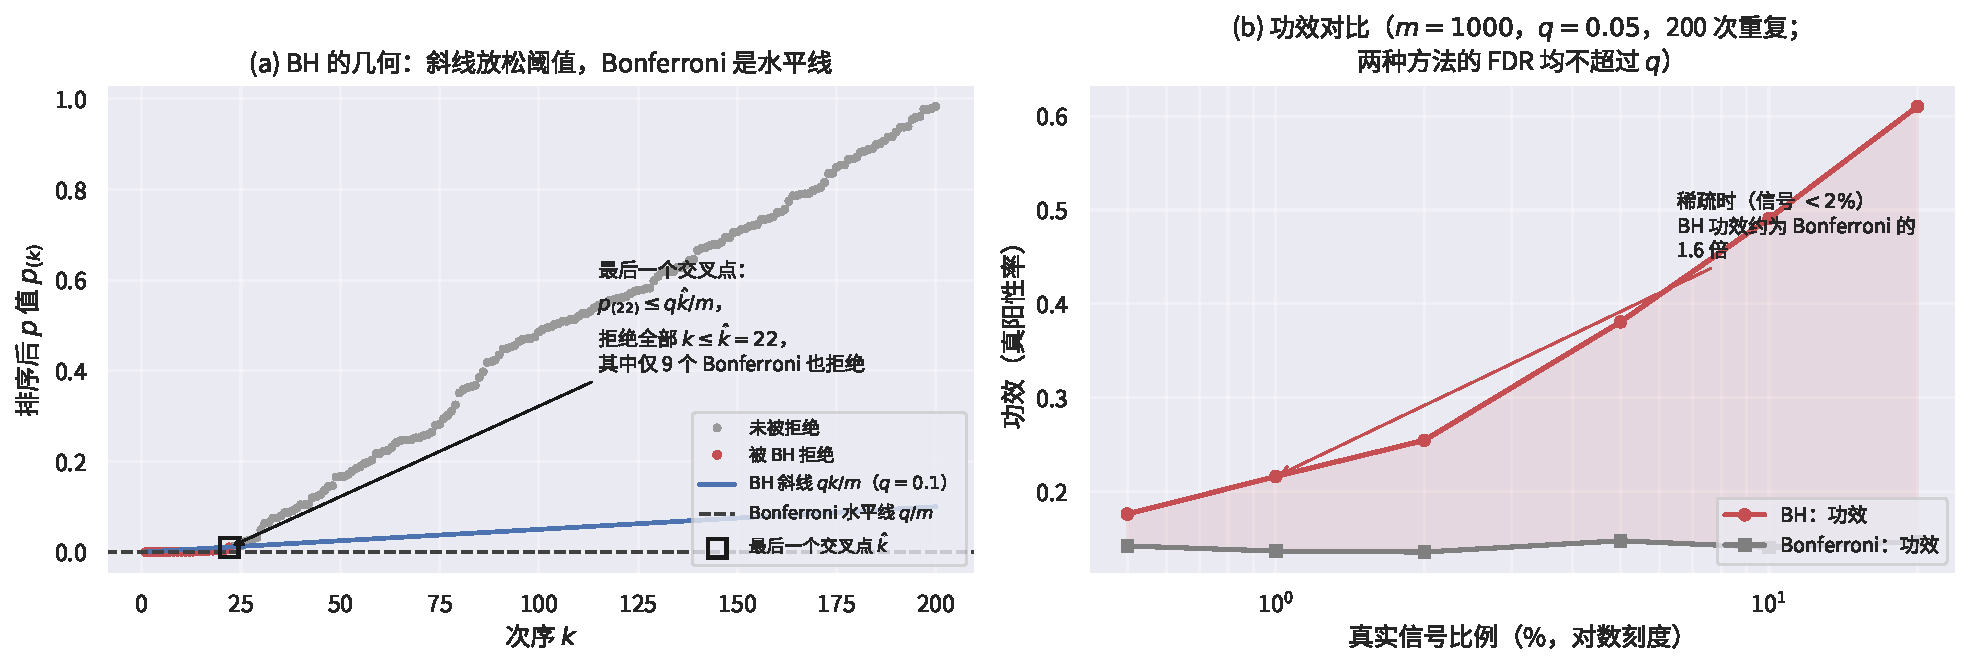
\includegraphics[width=\linewidth]{figures/ch7_fdr.pdf}
  \caption{(a) BH 的几何（一次模拟：$m=200$ 个独立检验，其中 30 个信号 $z_j \sim \mathcal{N}(3.2, 1)$，$q=0.1$）：排序 $p$ 值阶梯与斜线 $qk/m$ 的最后一个交叉点在 $\hat{k}=22$，拒绝全部 $k\le 22$；Bonferroni 的水平线 $q/m$ 只拒绝其中 9 个。(b) 功效模拟（$m=1000$，$q=0.05$，200 次重复）：信号比例从 $0.5\%$ 到 $20\%$（$z_j \sim \mathcal{N}(3,1)$），BH 的功效从 $0.18$ 升到 $0.61$，Bonferroni 的水平线被钉死在 $0.14$ 附近；信号比例为 $1\%$ 时 BH 功效约为 Bonferroni 的 $1.6$ 倍。两种方法的 FDR 实测均不超过 $q$（BH 在 $0.038$--$0.054$ 之间，Bonferroni 在 $0.0008$--$0.045$ 之间）——\textbf{斜线买到的功效没有多花一分钱错误率}。}
  \label{fig:ch7-fdr}
\end{figure}

\subsection{闭环：BH 是自适应的稀疏估计器}\label{sec:fdr-sparsity}

现在回到本书的主线——稀疏性。把单尾 $p$ 值换成 $z$ 分数 $z_j = \Phi^{-1}(1 - p_j)$，BH 程序等价于在有序 $z$ 分数上找一个\textbf{数据驱动的截断点}：拒绝 $z_{(j)} \ge \hat{t}$ 的假设。这个截断点不是预先给定的 $\sqrt{2 \log m}$，而是由数据自己「长」出来的——它长在哪里，取决于信号有多稀疏。

Abramovich、Benjamini、Donoho 与 Johnstone（2006）把这层观察变成了定理\cite{abramovich2006}。考虑稀疏正态均值模型
\[
  z_j = \theta_j + \varepsilon_j, \qquad \varepsilon_j \sim \mathcal{N}(0, 1),
  \qquad \#\{ j : \theta_j \neq 0 \} \le s \ll m,
\]
把 BH 在适当水平 $q$ 下的截断当作\emph{阈值估计器} $\hat\theta_j = z_j \cdot \ind{ z_j \ge \hat{t} }$（硬阈值）。其核心结论：\textbf{在稀疏度 $s$ 未知的情况下，这个由 FDR 控制规则定义的估计器自动达到与「知道 $s$」的 oracle 阈值相同的 minimax 风险率}——平方风险量级为 $2 s \log(m/s)$（相差常数因子），而不是非自适应阈值 $\sqrt{2 \log m}$ 给出的 $2 s \log m$。当 $s \ll m$ 时，$\log(m/s) \ll \log m$，这个差距是实质性的。

与第 \ref{sec:ggm-estimate} 节并排看，同一张面孔出现了两次：
\begin{center}
\begin{tabular}{@{}lll@{}}
\toprule
 & 稀疏估计（第 6 章） & FDR 检验（本节） \\
\midrule
对象 & 回归系数 $\bbeta$ 或均值 $\bm{\theta}$ & 一族假设 $H_1, \dots, H_m$ \\
机制 & $\ell_1$ 惩罚 / 软阈值 & 排序 $p$ 值 / BH 阈值 \\
自适应来源 & 惩罚参数 $\lambda$ 由交叉验证或 BIC & 截断点由斜线交叉自动定位 \\
稀疏性的角色 & 使估计在 $d \gg n$ 下仍可能 & 使 BH 阈值自动降到信号层 \\
\bottomrule
\end{tabular}
\end{center}
\textbf{控制假发现率不是估计之外的补丁，而是稀疏性假设在检验问题上的对偶表述}：「大多数系数是零」既让 lasso 能估计，也让 BH 能自适应地找到阈值。Donoho 的名字在第 6 章（压缩感知传统）与本节各出现一次，不是巧合——这是同一条「稀疏性 $\Rightarrow$ 阈值 $\Rightarrow$ 最优性」逻辑链的两端。

\subsection[回到回归 I：debiased lasso 的 $p$ 值与 BH]{回到回归 I：debiased lasso 的 $p$ 值经 BH，即控制系数的 FDR}\label{sec:fdr-regression}

流水线已经就位：第 \ref{sec:debiased} 节给出 $\sqrt{n}(\widetilde{\beta}_j - \beta_j)$ 的渐近正态性 \eqref{eq:asym-norm}，于是每个 $H_{0j}: \beta_j = 0$ 都有渐近 $p$ 值 $p_j$。把 $d$ 个 $p$ 值喂给 BH \eqref{eq:bh}，按定理 \ref{thm:bh}——只要 $p$ 值近似独立或正相关——\textbf{被拒绝的系数集合的假发现率就被控制在 $q$}。结合第 \ref{sec:beta-theta} 节的对应 $\beta_j = 0 \Leftrightarrow y \perp x_j \mid \x_{-j}$，这就是高维回归里「条件独立结构筛选」的标准终点：lasso 选候选边、debiased lasso 出 $p$ 值、BH 控可信度。

诚实的保留有三条，按本书惯例逐条披露：
\begin{enumerate}[label=(\roman*)]
  \item \textbf{$p$ 值是渐近的}。\eqref{eq:asym-norm} 是 $n \to \infty$ 的极限陈述，有限样本下 BH 的控制是近似的；$d$ 相对 $n$ 越大，近似越需要靠稀疏性条件托底。
  \item \textbf{相关性结构}。debiased 的 $p$ 值之间由设计矩阵的相关性决定。极端共线（第 \ref{sec:hd-break} 节的病态）可能破坏 PRDS 条件，实测 FDR 可以超调；一般相关下有更保守的 Benjamini--Yekutieli 修正\cite{benjamini2001}（把 $q$ 换成 $q / \sum_{j=1}^m j^{-1} \approx q / \log m$），代价是功效。
  \item \textbf{筛选与推断的对象一致性问题}。若用 lasso 先筛掉一部分变量、只对幸存者做检验，标准的 BH 理论不再直接适用（选择本身引入了额外随机性）——这正是下一节方法要绕开的坑。
\end{enumerate}

\subsection[回到回归 II：Knockoffs]{回到回归 II：Knockoffs——不依赖 $p$ 值的 FDR 控制}\label{sec:knockoffs}

Barber 与 Candès（2015）换了一条更彻底的路\cite{barber2015}：\textbf{不去造 $p$ 值再校正，而是在设计矩阵里人为构造「影子变量」，让对称性本身成为控制的支点}。对每列 $\x_j \in \R^n$，构造影子（knockoff）$\tilde{\x}_j$，使得\textbf{交换任意一对 $(\x_j, \tilde{\x}_j)$ 后，增广设计矩阵 $[\X\ \tilde{\X}]$ 的联合分布不变}（交换性）。高斯设计下有显式构造——它需要 $\X$ 列相关的二阶信息，即\textbf{又回到了第 \ref{sec:cov-prec} 节的协方差/精度矩阵}：影子变量按相关性「补齐」原变量，相关越强的变量，其影子越能以假乱真。（口径注记：原始 Barber--Candès 的\textbf{固定-$X$} 构造要求 $n \ge 2d$；本书描述的按二阶信息构造影子是 \textbf{model-X} 高斯版本，其高维构造至今仍是活跃研究方向。）

接着定义每个变量的特征重要性 $Z_j$ 与其影子的重要性 $\tilde{Z}_j$（例如 lasso 路径上该变量进入模型的次序），合成\textbf{带符号统计量}
\[
  W_j = Z_j - \tilde{Z}_j ,
\]
约定 $W_j$ 的符号表示「原变量胜过影子」。关键观察：在 $H_{0j}$（$\x_j$ 与 $\y$ 无关）下，$\x_j$ 与影子毫无差别，交换性给出
\begin{equation}\label{eq:knockoff-sym}
  W_j \ \overset{d}{=}\ -W_j
  \qquad (H_{0j} \text{ 下，以其他变量为条件}),
\end{equation}
即\emph{零假设变量的 $W_j$ 关于 $0$ 对称}，而真实信号变量的 $W_j$ 倾向于取大正值。于是「负 $W$ 的个数」就成了「假发现的个数」的\textbf{对称性估计}：按 $|W_j|$ 从大到小， knockoff+ 程序取阈值
\begin{equation}\label{eq:knockoff}
  T = \min\Big\{ t > 0 :\ \frac{ 1 + \#\{ j : W_j \le -t \} }{ \#\{ j : W_j \ge t \} } \le q \Big\},
  \qquad
  \text{拒绝 } \{ j : W_j \ge T \}.
\end{equation}
分子里那个「$1+$」是对随机性的过离散校正；而 \eqref{eq:knockoff-sym} 保证每个被误拒的变量以 $1/2$ 的概率贡献一个负镜像——这正是定理证明的支点。结论：在任意模型（不需要线性、不需要渐近）下，
\[
  \mathrm{FDR} \le q .
\]

两条路线并排看，各司其职：
\begin{center}
\begin{tabular}{@{}lll@{}}
\toprule
 & BH + debiased lasso（第 \ref{sec:fdr-regression} 节） & Knockoffs（本节） \\
\midrule
控制支点 & $p$ 值的渐近正态性 & 设计矩阵的交换对称性 \\
模型假设 & 需要（线性 + 稀疏 + 渐近） & 不需要（模型无关） \\
有限样本保证 & 近似（渐近成立） & \textbf{精确}（有限样本） \\
额外代价 & debias 需要的 nodewise 估计 & 构造影子变量（固定-$X$ 构造需 $n \ge 2d$；model-X 需已知或可估特征分布） \\
\bottomrule
\end{tabular}
\end{center}

至此，「可信的科学断言」三件套齐备：debiased lasso 给\textbf{单个}系数的 $p$ 值（第 \ref{sec:debiased} 节），BH 给\textbf{一页} $p$ 值的 FDR 控制（本节之前），knockoffs 给\textbf{变量选择}的、模型无关的 FDR 控制（本节）。Candès 与 Donoho 在前言里被致敬，是因为回归的现代可信度理论恰好由他们两脉写成——一个负责「稀疏使估计可能」，一个负责「对称使推断可信」。

\begin{keybox}[本章要点]
\begin{itemize}
  \item 多重检验下 Bonferroni 控制 FWER 但阈值 $\alpha/m$ 随 $m$ 线性收紧、功效崩塌；FDR $= \E[V/\max(R,1)]$ 允许「发现多时容忍少量假的」，是探索性筛选的正确货币（\ref{sec:fdr-problem} 节）；
  \item BH 程序 $=$ 排序 $p$ 值与斜线 $qk/m$ 的最后一个交叉点；独立（或 PRDS）下 $\mathrm{FDR} \le q\, m_0/m \le q$（定理 \ref{thm:bh}）；
  \item 闭环：BH 阈值是对 $z$ 分数的自适应稀疏估计，稀疏度未知时达到 oracle 级别的 minimax 率\cite{abramovich2006}——控制假发现率与稀疏估计是同一枚硬币；
  \item 回归流水线：debiased lasso 出 $p$ 值、BH 控 FDR——但渐近近似与共线性是诚实披露的弱点；knockoffs 用影子变量的交换对称性给出模型无关、有限样本精确的 FDR 控制\cite{barber2015}。
\end{itemize}
\end{keybox}

\begin{exercise}\label{ex:bh-hand}
$m = 5$、$q = 0.1$，五个 $p$ 值（已排序）为 $0.001,\ 0.02,\ 0.04,\ 0.09,\ 0.3$。逐步执行 BH：写出每个 $k$ 的阈值 $qk/m$、判定、$\hat{k}$ 与最终拒绝集；再与 Bonferroni（阈值 $q/m$）及「逐个检验水平 $q$」三者的拒绝集比较。
\end{exercise}

\begin{exercise}\label{ex:bh-bonf}
(a) 证明 $\mathrm{FDR} \le \mathrm{FWER}$，并由此得出「控制 FWER 的任何程序（如 Bonferroni）必然控制 FDR」；(b) 证明 Bonferroni 在水平 $q$ 下的拒绝集是 BH 在水平 $q$ 下拒绝集的子集；(c) 设 $m = 10^5$ 个独立检验，其中 $200$ 个信号的 $z_j \sim \mathcal{N}(5, 1)$（双侧 $p$ 值），$q = 0.05$。估计 Bonferroni 的每检验阈值与功效，说明 BH 在 $\hat{k} \approx 200$ 处的阈值比它宽松多少、以及为什么此时 BH 的功效趋近 $1$ 而 Bonferroni 远不至此。
\end{exercise}

\begin{exercise}[证明梗概，较难]\label{ex:bh-proof}
在\textbf{全部 $m$ 个假设为真}且 $p$ 值\textbf{相互独立}的条件下，证明 $\Prob( \exists k : p_{(k)} \le qk/m ) \le q$（全零时 $\mathrm{FDR}$ 等于这个概率，故定理 \ref{thm:bh} 的最坏情形成立）。按以下骨架补全：(i) 对 $m$ 归纳，$m = 1$ 显然；(ii) 关键一步：以最大次序统计量 $p_{(m)}$ 是否 $\le q$ 分情况，利用「固定 $p_{(m)} = u$ 时，其余 $m-1$ 个是 $m-1$ 个独立 $U(0, u)$ 变量除以 $u$」的事实，把事件改写成关于 $m-1$ 个均匀变量的同类事件，并验证水平参数从 $q$ 变成 $q/u \cdot (u) = q$ 的恒等；(iii) 合并两种情况。
\end{exercise}

\begin{exercise}\label{ex:knockoff}
(a) 由交换性严格说明：在 $H_{0j}$ 下，把 $\x_j$ 与 $\tilde{\x}_j$ 全局交换后统计量向量 $(W_1, \dots, W_m)$ 的联合分布不变，而这使 $W_j$ 变号——由此得出 \eqref{eq:knockoff-sym}（提示：$H_{0j}$ 下 $\y$ 不依赖 $\x_j$，交换不改变回归问题）；(b) 解释为什么 \eqref{eq:knockoff} 分母里的 $\#\{j : W_j \ge t\}$ 是「$|W|$ 超过 $t$ 的发现数」，而分子（除 $1+$ 外）的 $\#\{j : W_j \le -t\}$ 是它的\textbf{假发现数估计}——对称性如何把这个估计变成上界期望的支点。
\end{exercise}
